\chapter{Concepts}
\label{chapter:ConfConcepts}
The solution to the problems outlined in Chapter \ref{chapter:ConfTask} can be achieved with
the help of the Eclipse plug-in technology described in Chapter \ref{chapter:ConfTechnology}.

This chapter explains the solutions in the same structure as Chapter \ref{chapter:ConfTask}.
That means that it will start by introducing solutions to the problem of how save the new
configuration properties into the existing execution files. In addition the chapter will
explain ways to enable the user to set up a series of default configurations. The last
section of this chapter will explore possibilities of how to make it easier to load
previously saved schedules.

\section{Configurations}
\label{section:ConfConceptsConf}
\index{Execution file}
The first approach to save additional configuration information in the execution files (see Section \ref{section:IntroExecution}) would
be to actually modify the format of those files and write the information into them.
This would most likely be the easiest approach but would destroy backward compatibility of
those files since the basic Execution Manager would not know how to deal with the modified files.

The approach taken in this thesis is based on the list of DataComponents (see Section \ref{section:IntroDataComponent}). Each execution file 
carries a list of its own DataComponents and their properties to ensure
that the component are properly initialized the next time the execution is loaded. That list
can be loaded even if there are DataComponents contained in it that are not present in the current
runtime configuration. The Execution Manager will show a warning indicating that it doesn't know the given
component but proceed to load the rest of the execution. 

These DataComponents basically just carry a list of KiemProperties which are
basically (key, value) pairs. Hence, they are suited well for storing simple information like the value
of a text field.

To solve the problem a new type of DataComponent will have to be constructed and registered through
the extension point in the Execution Manager . This ensures that the component can be added to any execution
file. The Execution Manager  ensures that all properties contained in our component will be saved with
the execution file and loaded the next time the file is opened. After that the configuration plug-in has 
find the component inside the DataComponent list, get the properties saved inside it
and set them inside the Execution Manager.

\subsection{Default Configuration}
\label{section:ConfConceptsDefaultConf}
\index{Default Configuration}
In order to provide a place to manage the default configurations we will be
using the Eclipse preference pages.

The root page for the Execution Manager should contain the basic settings for the \ac{KIEM} itself like
the aimed step duration, timeout and the view elements of the Configuration plug-in.

\begin{figure}[MSPLayoutPreferencePage]
  \centering
  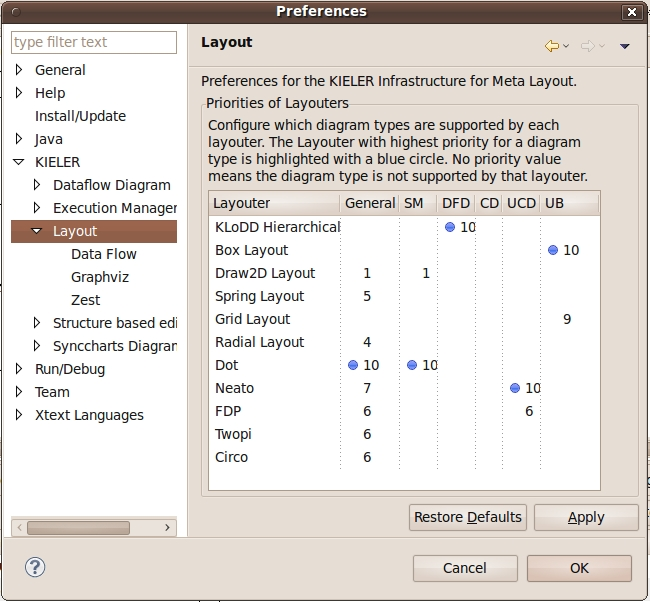
\includegraphics[scale=.5]{MSPLayoutPreferencePage.jpg}
  \caption[Layout Preference Page by Miro Sp\"onemann]%
  {Layout Preference Page by Miro Sp\"onemann\protect}
  \label{fig:MSPLayoutPreferencePage}
\end{figure}

Then we will construct another page for managing the different schedules
and their editors. For that we will adapt the LayoutPreferencePage by Miro Sp\"onemann
as seen in Figure \ref{fig:MSPLayoutPreferencePage}. The original preference page
displays a table where different layouters can be assigned priorities for different diagram
types. This is similar to the problem that needs to be solved in this thesis. The diagram types
can be mapped to our editors and the layouters will be replaced by the list of saved schedules.
That way the modified preference page can be used to assign priorities to schedules for
different editors. The priorities can then be used to sort the schedules matching
the currently opened editor.

The last page will be used to allow the user to set up his own properties and give them
default values.

The values entered in those pages will be stored inside the Eclipse preference
store (see Section \ref{section:TechPreferenceStore}).

\section{Easier Configuration loading}
\label{section:ConfConceptsEasyLoading}
For easier configuration loading we will add two ComboBoxes to the existing
tool bar inside the \ac{KIEM} view.

One of them will display the list of recently used schedules the other one the
list of schedules that work for the currently active editor.

As soon as the user opens a new execution file through the normal workspace
view we will be notified of that event by the Execution Manager. We will then create a new
schedule and store the path to the execution file in it along with the editor
that was opened at the time that the schedule was created. The new schedule will
also be added to the list of recently used schedules that we maintain through the 
use of the Eclipse preference store.

When the user selects one of the previously saved schedules in one of the
ComboBoxes we will retrieve the saved path and offer it to the KiemPlugin to
load it in the hopes that the execution file is still in the same location and
wasn't deleted, renamed or moved by the user.
